\documentclass[letterpaper,journal]{IEEEtran}
\usepackage{amsmath,amsfonts,amssymb}
\usepackage{array,graphicx,xcolor,booktabs,tabularx}
\usepackage{url}
\hyphenation{op-tical net-works semi-conduc-tor IEEE-Xplore}

\newcommand{\agent}[1]{%
    \textcolor{red}{\textbf{[Agent:} #1\textbf{]}}%
}
\begin{document}
\title{Nonintrusive Cross-Motor Detection and Severity Assessment of False-Data-Injection Attacks in Heterogeneous Inverter-Fed Drives
}

\author{%
    Abolfazl Najar, He Yang, Jin Ye,~\IEEEmembership{Senior Member,~IEEE},  Ping Ma and WenZhan Song,~\IEEEmembership{Senior Member,~IEEE}%

    \thanks{Abolfazl Najar, He Yang, Jin Ye, and WenZhan Song are with the College of Engineering, University of Georgia, Athens, GA 30602, USA (e-mail: najar@uga.edu; heyang95@uga.edu; jin.ye@uga.edu; wsong@uga.edu).}%
    
    \thanks{Ping Ma is with the Department of Statistics, University of Georgia, Athens, GA 30602, USA (e-mail: pingma@uga.edu).}%
    
    \thanks{Corresponding author: Jin Ye (e-mail: jin.ye@uga.edu).}%
    
}

\maketitle

\begin{abstract}
This paper evaluates false-data-injection attack (FDIA) detection and injected-bias severity assessment in heterogeneous inverter-fed drives using trusted motor-terminal or point-of-common-coupling (PCC) measurements. Low-frequency, high-frequency, and time-domain features are combined with an InceptionTime classifier. Laboratory data comprise 18 recordings from an alternating current induction motor (ACIM) and a permanent magnet synchronous motor (PMSM), covering three speeds and three load settings. Training, validation, and testing use disjoint recordings and episodes, with three repeated holdouts. Mean binary detection accuracy is 87.41\% for motor-side sensing and 80.78\% for PCC sensing; corresponding four-class severity balanced accuracies are 90.81\% and 55.62\%. The proposed model attains the highest mean PCC balanced accuracy among the evaluated baselines, although it does not lead every severity metric. The PCC severity model identifies 61.39\%, 85.08\%, and 88.09\% of low-, medium-, and high-bias attacks as attacks, respectively, with a 37.23\% normal false-alarm rate. Supervised PMSM-to-ACIM fine-tuning reaches 91.38\% PCC balanced accuracy at a nominal 20\% target adaptation budget, while the reverse direction remains difficult. Removing high-frequency features reduces PCC processing time from 22.37 to 12.32~ms with similar detection balanced accuracy. These results characterize the capabilities and limitations of PCC monitoring on the tested platform under additive feedback-bias attacks.
\end{abstract}

\begin{IEEEkeywords}
False-data-injection attack, point of common coupling, inverter-fed motor drives, heterogeneous motor drives, nonintrusive monitoring, cross-motor adaptation, severity assessment, cyber-physical security
\end{IEEEkeywords}

\section{Introduction}
\label{sec:introduction}
 
\IEEEPARstart{F}{DIA} detection and severity assessment are important in networked motor-drive systems, where manipulated sensor feedback can degrade control performance and cause unsafe operation~\cite{Ghaderi2021A}. Increasing drive connectivity makes timely detection of sensor-oriented cyber attacks essential for resilient operation~\cite{Yang2022Fast,Yang2024Enhanced}.
Current signals are attractive for FDIA monitoring because they are easy to acquire, strongly coupled to electromechanical dynamics, and have been shown to reveal sensor-integrity attacks in motor drives~\cite{7944701, YangVulnerability}. However, most existing studies emphasize terminal-side sensing, operate on a single machine domain, or assume sufficient labeled data for supervised training. These assumptions limit practicality in heterogeneous deployments where different motor types, sensing locations, and data availability constraints all affect performance.
Motivated by these limitations, this work experimentally evaluates FDIA detection in a heterogeneous motor-drive setting involving both ACIM and PMSM domains. The study evaluates binary detection, four-level injected-bias assessment, cross-domain transfer, and processing cost for converter-fed industrial loads connected at a shared electrical interface. The framework combines low-frequency (LF), high-frequency (HF), and time-domain (TD) electrical features with an InceptionTime classifier, and compares motor-terminal and PCC sensing.

\subsection{Challenges at PCC in Heterogeneous Multi-Motor Systems}
\label{sec:pcc_challenges}

From a deployment perspective, motor-terminal measurements provide cleaner machine-specific signatures, whereas PCC measurements are more scalable and non-intrusive. PCC sensing is attractive because it avoids direct motor-terminal instrumentation and is compatible with shared electrical infrastructure~\cite{7271086}. However, PCC currents are affected by converter harmonics, network interactions, and load aggregation. Consequently, PCC attack signatures are weaker and less separable than motor-terminal signatures~\cite{10005067}.
The problem becomes more difficult in heterogeneous multi-motor settings. ACIM and PMSM systems exhibit different current characteristics even under the same attack framework, which introduces a substantial domain shift between source and target deployments. Consequently, a detector trained on one motor family may generalize poorly to the other unless explicit adaptation is used. Therefore, this study evaluates in-domain performance, source-only transfer, few-shot adaptation, and transfer-direction asymmetry.
\subsection{Contributions}
\label{sec:contributions}
The main contributions of this work are as follows:

\begin{itemize}
\item \textbf{Evaluated} nonintrusive PCC-based FDIA detection on a heterogeneous ACIM/PMSM laboratory platform using whole-recording holdouts that also keep all constituent episodes disjoint.
\item \textbf{Quantified} the distinction between exact injected-bias classification and detecting an attack of a given bias level, reporting classwise recall together with normal false alarms and repeated-holdout variability.
\item \textbf{Compared} source-only transfer, supervised adaptation, and target-only training, and measured the accuracy--processing-cost tradeoff of LF/HF/TD representations and validation-ranked feature subsets.
\end{itemize}

The remainder of this paper is organized as follows: Section~\ref{sec:relatedWorks} reviews related literature. Section~\ref{sec:system_data} describes the physical system and dataset construction, while Section~\ref{sec:method} details the proposed FDIA detection framework and feature pipeline. Experimental results and cross-domain adaptations are reported in Section~\ref{sec:results}. Section~\ref{sec:realtime} analyzes real-time deployment and latency, followed by a discussion of tradeoffs in Section~\ref{sec:discussion}. Section~\ref{sec:conclusion} concludes the paper.

\section{Related Work}
\label{sec:relatedWorks}

FDIA detection has been studied extensively in smart grids and broader cyber-physical systems (CPS), but the assumptions in that literature do not transfer cleanly to inverter-fed motor drives. Many grid- and CPS-oriented approaches rely on state estimation, observer-based detection, invariant analysis, adaptive neuro-fuzzy models, or graph-based learning~\cite{7438916,basati2022fdi,nath2022quickest,beg2017fdia,sargolzaei2020fdia,10016905}. These studies demonstrate strong FDIA-detection capability at the system level, but they are generally not designed for drive-level current monitoring or for deployment at a shared point of common coupling (PCC).

Motor-drive-specific studies are more closely related to the present work. Prior work has shown that current signals can support effective FDIA detection in electric-drive systems and that transfer learning can improve performance when labeled data are limited~\cite{Yang2022Fast,Yang2024Enhanced}. Related industrial-IoT monitoring studies have also considered cyber-detection in machine-monitoring settings~\cite{423563247547}. However, these studies mainly rely on motor-terminal sensing, single-motor settings, or closely related operating domains, and therefore provide limited evidence for heterogeneous cross-motor transfer.


The main gap is not FDIA detection in general, which has been widely studied in smart grids and cyber-physical systems, but nonintrusive PCC-based monitoring for heterogeneous inverter-fed motor-drive systems. In particular, the existing literature does not clearly establish: 1) how PCC sensing compares with motor-side sensing for low-severity current-feedback FDIAs, 2) whether PCC measurements support reliable multi-level severity assessment rather than only binary detection, given that attack signatures become weaker and less separable under signal aggregation and harmonic distortion, and 3) how detection performance transfers between heterogeneous ACIM and PMSM domains when labeled target-domain data are limited. The contribution is a comparative experimental assessment rather than a new neural-network architecture. This work addresses these three questions experimentally on a shared ACIM/PMSM platform using multi-scale features, in-domain evaluation, source-only cross-domain transfer, and few-shot target-domain adaptation.


        


      
              


\section{System and Data}
\label{sec:system_data}
\subsection{Experimental Platform: ACIM/PMSM and PCC Sensing}
\label{sec:experimental_platform}

Fig.~\ref{fig:system_schematic} illustrates the overall setup, including the shared PCC, the two drive branches, the ACIM and PMSM loads, the sensing locations, and the FDIA injection points in the control/feedback paths. The experimental platform consists of a heterogeneous two-motor industrial setup including one ACIM branch and one PMSM branch. Both branches are supplied from a common upstream electrical interface, enabling measurements at the PCC in addition to motor-side measurements. This setup enables comparison of motor-terminal and PCC sensing under heterogeneous ACIM/PMSM dynamics.
The dataset contains 540 scheduled attack episodes (270 for each motor), formed by repeating 30 bias patterns over nine speed/load combinations per motor. These episodes are not 540 independent motor installations. The experiments cover three speed operating points, namely 900, 1100, and 1300 rpm. 

Two measurement streams were used throughout this study. The first stream corresponds to motor-side measurements, referred to as \emph{motor} in the remainder of the paper. The second stream corresponds to PCC-side measurements, referred to as \emph{PCC}. The PCC stream is the primary deployment-oriented sensing location because it avoids dedicated sensors at each machine. The measured signals and channel counts associated with the motor-side and PCC-side streams are summarized in Table~\ref{tab:measurement_streams}.

\agent{restore the previous version of this figure from main.tex If anything needs to be revised in the figure let me know. }
\begin{figure*}[t]
\centering
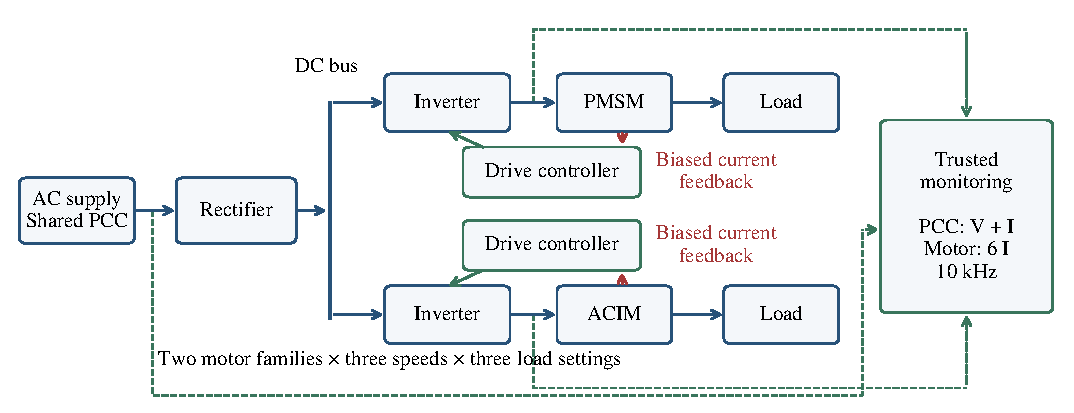
\includegraphics[width=\linewidth]{figs_revised/figure1_platform.pdf}
\caption{Shared-rectifier, two-branch inverter-fed drive platform and monitoring locations. Dashed red paths identify the attacked controller-current feedback; green dashed taps provide separate monitoring measurements assumed trusted.}
\label{fig:system_schematic}
\end{figure*}

\subsection{Attack Model, Sensing Assumptions, and Labels}
\label{sec:attack_labels}

In the testbed, the FDIA is injected into the controller's phase-current feedback path. The PCC and motor-side monitoring sensors are used as trusted measurements to record the physical response of the drive system under attack. 
The monitoring sensors are isolated from the compromised controller feedback path. Thus, PCC sensing represents the nonintrusive monitoring case, while motor-side sensing serves as a performance reference. Replay, denial-of-service, monitoring-sensor attacks, and malicious command manipulation are outside the scope of this study.

Let $\mathbf{i}_{abc}(t)=[i_a(t),i_b(t),i_c(t)]^\top$ denote the true three-phase current-feedback vector in the controller's per-unit representation, and let $\tilde{\mathbf{i}}_{abc}(t)$ denote the corrupted current-feedback vector received by the motor controller. During an attack interval, the FDIA is modeled as an additive phase-current bias:
\begin{equation}
\tilde{\mathbf{i}}_{abc}(t)
=
\mathbf{i}_{abc}(t)+\boldsymbol{\alpha},
\qquad t\in[t_{\mathrm{on}},t_{\mathrm{off}}],
\label{eq:fdia_model}
\end{equation}
Here, \(\boldsymbol{\alpha}=[\alpha_a,\alpha_b,\alpha_c]^\top\) denotes the injected per-unit bias vector, with \(\boldsymbol{\alpha}=\mathbf{0}\) outside the attack interval. The tested nonzero bias magnitudes range from \(0.0005\) to \(0.0050~\mathrm{pu}\), corresponding to \(0.05\%\)--\(0.5\%\) current-feedback bias. Percentages refer to the nominal controller feedback base; no absolute ampere or torque calibration is inferred from them. The term severity denotes injected bias magnitude, not measured physical harm. Attack severity is measured by the largest absolute injected phase-current bias, 
\(s=\|\boldsymbol{\alpha}\|_\infty\).

For binary FDIA detection, each window is labeled as
$y_{\mathrm{fdia2}}=1$ if $s>0$ and $y_{\mathrm{fdia2}}=0$ otherwise. 
For four-class severity assessment, the label is defined as
\begin{equation}
y_{\mathrm{severity4}} =
\begin{cases}
0, & s=0 \quad \text{(normal)},\\
1, & 0.0005 \leq s \leq 0.0015 \quad \text{(low)},\\
2, & 0.0020 \leq s \leq 0.0035 \quad \text{(medium)},\\
3, & 0.0040 \leq s \leq 0.0050 \quad \text{(high)}.
\end{cases}
\label{eq:severity_bins}
\end{equation}
The bins apply to the tested discrete bias values and are not standardized safety thresholds. Cases 21--30 have $s=0.0050$ throughout because phase A remains fixed; all belong to the high-bias class. The resulting attack-window counts are 5,400 low, 7,200 medium, and 14,400 high.
Table~\ref{tab:cyberattack_dataset_structure} summarizes the swept single-phase, equal two-phase, and fixed-plus-swept two-phase FDIA cases. Across three speeds, three load settings, and two motor types, the dataset contains 540 total attack cases. Each recording contains 30 consecutive 20-s episodes, with 10~s normal operation followed by 10~s FDIA operation. After the scheduled 600~s, the injected bias was zero and the motor continued running. All 6,054 complete post-schedule windows are retained as normal, giving 33,054 normal and 27,000 attack windows in total.

\begin{table}[t]
\centering
\footnotesize
\caption{FDIA dataset structure.}
\label{tab:cyberattack_dataset_structure}
\renewcommand{\arraystretch}{1.12}
\begin{tabular}{c c c c}
\hline
Cases & Phases & Bias Pattern & Total \\
\hline
1--10  & A   & $\alpha_a$: $0.0005$--$0.0050$ & 180 \\
11--20 & A,B & $\alpha_a=\alpha_b$: $0.0005$--$0.0050$ & 180 \\
21--30 & A,B & $\alpha_a=0.0050$, $\alpha_b$: $0.0005$--$0.0050$ & 180 \\
\hline
\multicolumn{3}{r}{Overall} & 540 \\
\hline
\end{tabular}
\vspace{1mm}
\begin{flushleft}
\footnotesize Each case group is evaluated over 3 speeds, 3 load settings, and 2 motor types. For all cases, unspecified phase biases are zero.
\end{flushleft}
\end{table}


\subsection{Data Acquisition and Operating Conditions}
\label{sec:data_acquisition}

Electrical measurements were acquired from the testbed using a National Instruments cDAQ-9185 chassis and a custom data-collector interface board. The interface board routed synchronized motor-side and PCC-side analog channels to the acquisition system. Three brake-excitation settings were tested for each machine: 1--3~V for the ACIM branch and 2--4~V for the PMSM branch. Because torque was not directly measured, these brake-excitation voltages are used as load-condition labels. All channels were sampled at 10~kHz and stored in TDMS format. For learning-based analysis, each record was segmented into non-overlapping 0.2~s windows containing 2{,}000 samples. Non-overlap prevents reuse of raw samples between adjacent windows, but does not remove within-recording dependence. Therefore, each entire recording, including its 30 episodes and post-schedule normal segment, is assigned to one partition. For each motor, five recordings are used for training, two for validation, and two for testing. Three seeds (1234, 2234, and 3234) change both the recording assignment and initialization. All feature normalization statistics are fitted using training recordings only. For example, all windows from one ACIM speed/load recording stay together; an adjacent attack episode cannot appear in a different partition. The holdouts assess new recorded operating combinations on the same apparatus; recordings can recur across repeats. The resulting dataset dimensions, input configurations, severity-label distributions, and evaluation protocols are summarized in Table~\ref{tab:evaluation_protocols}.
\agent{I think previous version of figure in the main file was better. bring back that one. also these lines are not clear. what 6/3 means I believe you can increase the wording

Seed 1234 windows 33,718 / 13,279 / 13,057
Seed 2234 windows 33,275 / 13,250 / 13,529
Seed 3234 windows 33,560 / 13,227 / 13,267
Transfer: source train / val. 6 / 3 recordings
Transfer: target pool / test 6 / 3 recordings
Target episode-group budgets 2 / 9 / 18 / 36 of 180}
\begin{figure*}[t]
\centering
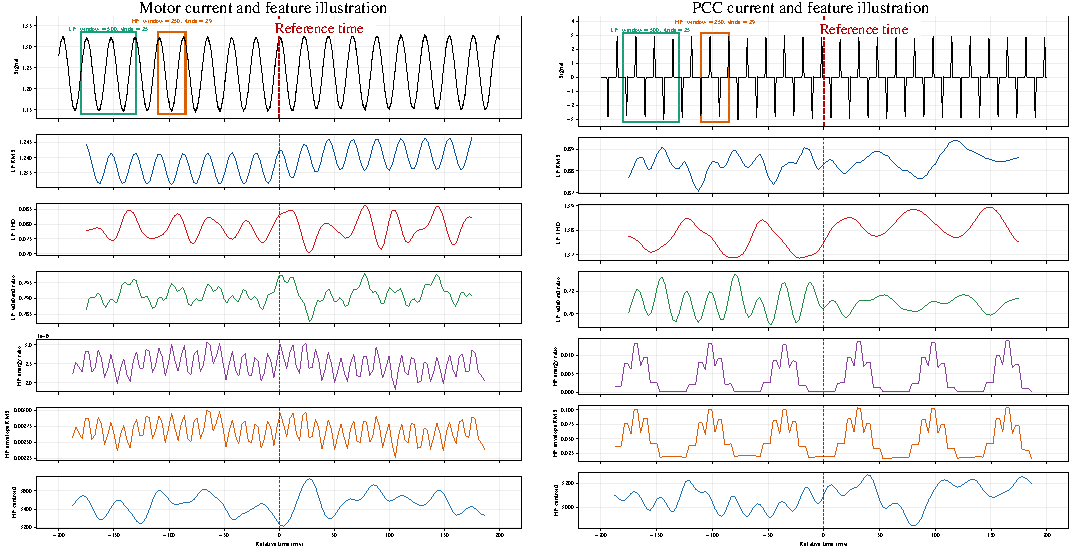
\includegraphics[width=\linewidth]{figs_revised/figure2_feature_example.pdf}
\caption{Descriptive motor-current and PCC-current examples around the first scheduled attack onset in the first alphabetic held-out ACIM recording for seed 1234. LF/TD frames use 500 samples with stride 25; HF frames use 250 samples with stride 29. The vertical line marks the documented onset; feature trajectories are shown at frame centers for illustration, not as causal detector outputs. Signal amplitude is in recorded acquisition units.}
\label{fig:lfhf_motor_pcc_examples}
\end{figure*}

\agent{totally I liked the severity4 and fdia2 more than this version. Is there any way to use similar thing or better way to show task? }
\begin{table}[t]
\centering
\caption{Measurement streams used for monitoring.}
\label{tab:measurement_streams}
\renewcommand{\arraystretch}{1.15}
\begin{tabular}{l c c}
\hline
Stream & Measured signals & Channels \\
\hline
Motor-side & ACIM and PMSM phase currents & 6 \\
PCC-side   & PCC voltage and current & 2 \\
\hline
\end{tabular}
\end{table}                       

\agent{for this figure check the style of previous version and use that. Do that for all tables. Try to keep same style since it is much easier to read. If anyother or data is added you can add them in appropriate column and row. }
\begin{table}[t]
\centering
\footnotesize
\caption{Dataset dimensions and recording-disjoint evaluation protocols.}
\label{tab:evaluation_protocols}
\renewcommand{\arraystretch}{1.12}
\setlength{\tabcolsep}{3pt}
\begin{tabular}{lc}
\hline
Parameter & Value / configuration \\
\hline
Complete windows & 60,054 (0.2 s each) \\
Recordings / episodes & 18 / 540 scheduled \\
Post-schedule normal windows & 6,054 \\
Motor distribution & ACIM 30,204; PMSM 29,850 \\
Binary classes & Normal 33,054; attack 27,000 \\
Severity classes & Normal 33,054; low 5,400 \\
 & Medium 7,200; high 14,400 \\
Features / channel & 18 LF + 11 HF + 8 TD \\
Motor input & $61\times222$ (6 channels) \\
PCC input & $61\times74$ (2 channels) \\
Main split: train / val. / test & 10 / 4 / 4 recordings \\
Seed 1234 windows & 33,718 / 13,279 / 13,057 \\
Seed 2234 windows & 33,275 / 13,250 / 13,529 \\
Seed 3234 windows & 33,560 / 13,227 / 13,267 \\
Transfer: source train / val. & 6 / 3 recordings \\
Transfer: target pool / test & 6 / 3 recordings \\
Target episode-group budgets & 2 / 9 / 18 / 36 of 180 \\
\hline
\end{tabular}
\par\smallskip\begin{minipage}{\linewidth}\footnotesize Both motor types occur in every main partition. No recording or episode crosses partitions within a repeat. Tail segments follow their parent recordings.\end{minipage}
\end{table}

\section{The Proposed Method}
\label{sec:method}

\subsection{LF/HF Feature Extraction Pipeline}
\label{sec:lfhf_features}


To represent both slow electromechanical behavior and faster attack-induced disturbances, a two-scale LF/HF feature pipeline was applied independently to each measured channel. For every sample, a 2{,}000-point outer window was first extracted from the raw 10~kHz recording. Within this outer window, two parallel sliding analyses were performed. The LF branch uses a 500-sample window with a stride of 25 samples, while the HF branch uses a 250-sample window with a stride of 29 samples. The LF and HF settings both produce 61 time steps, enabling concatenation into one temporal feature tensor. 
Fig.~\ref{fig:lfhf_motor_pcc_examples} illustrates representative attack-onset responses and the corresponding LF/HF windows. In both cases, the raw signal is shown around the attack-transition instant, and representative LF and HF windows are overlaid to illustrate the two-scale extraction procedure. The motor-side signals exhibit stronger and more localized variations, whereas PCC-side responses are more distributed due to their aggregated nature.

In total, 37 features were extracted per channel, including 18 LF spectral features, 11 HF spectral/envelope features, and 8 TD features. The LF branch targets slow electromechanical changes, fundamental-frequency behavior, harmonic distortion, sideband effects, and low-band energy redistribution. The HF branch captures higher-frequency redistribution and envelope-related changes that may appear during small current-feedback FDIAs. The TD features provide complementary sensitivity to amplitude variation, impulsiveness, waveform asymmetry, and short-term signal complexity.
Their relative contributions are evaluated through fixed-family ablations; improved separability is assessed empirically rather than assumed for every feature family.

\subsection{Inception-Based Detection Model}
\label{sec:inception_model}

The extracted LF/HF tensors were modeled using a one-dimensional InceptionTime architecture~\cite{fawaz2020inceptiontime} for multivariate time-series classification. The input dimension is $(61,222)$ for the motor stream and $(61,74)$ for the PCC stream. As illustrated in Fig.~\ref{fig:inceptiontime_architecture}, the network uses bottleneck compression, parallel one-dimensional convolutional kernels of lengths 39, 19, and 9, residual shortcuts, global average pooling, and a dense output layer. Motor and PCC models used stream-specific hyperparameters selected by validation balanced accuracy. The Inception-based design is well suited to the proposed LF/HF representation because the extracted features retain temporal ordering across the 61-step sequence. This preserves temporal interactions among LF, HF, and TD features.

\agent{previous version of figures was much better. tell me to revise them if it needs any revise in any block.}
\begin{figure*}[t]
\centering
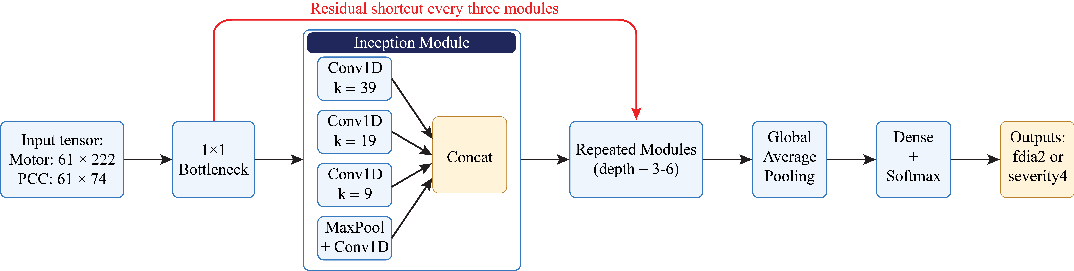
\includegraphics[width=\linewidth]{figs_revised/figure3_architecture.pdf}
\caption{Implemented InceptionTime classifier. Each module has three temporal convolutions and a max-pooling projection branch, followed by concatenation, batch normalization (BN), and ReLU. A projected residual shortcut is added after each group of three modules; depth and other settings are selected separately for each task, stream, and repeat.}
\label{fig:inceptiontime_architecture}
\end{figure*}

\subsection{Architecture of Online FDIA Detection and Attack-Severity Estimation}
\label{sec:AnomalyDetection}
The proposed pipeline supports online monitoring from trusted motor-terminal currents or PCC voltage/current measurements. Figure~\ref{fig:Online-algorithem} illustrates the overall architecture of the proposed monitoring pipeline. In the intended monitoring setting, fixed-length windows of electrical measurements are acquired from either the motor terminals or the PCC, passed through the LF/HF feature-extraction stage, and then evaluated by the selected learning model to produce anomaly or severity decisions. The measurement, feature-extraction, and inference stages are modular, allowing the same pipeline to operate with motor-side or PCC inputs and supporting feature pruning, reduced-input models, and cross-motor adaptation. The framework provides alarms, severity indicators, and logs for supervisory systems; automatic mitigation is outside the scope. The same architecture is used for binary detection and severity classification. Binary detection is the primary PCC deployment task; severity estimates provide secondary diagnostic information. The experimental results in later sections show that motor-terminal sensing provides cleaner discriminative signatures, whereas PCC sensing offers a less intrusive sensing option for the tested setup.

\begin{figure*}[t]
\centering
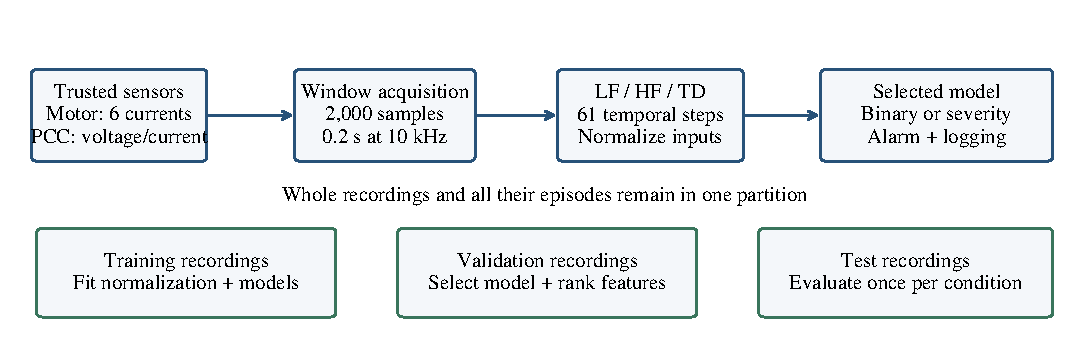
\includegraphics[width=\linewidth]{figs_revised/figure4_pipeline.pdf}
\caption{Monitoring pipeline and evaluation boundaries. A 0.2-s acquisition precedes feature computation and inference. Normalization and model fitting use training data; model selection and feature ranking use validation data. Test recordings are reserved for evaluation. Automatic mitigation is not evaluated.}
\label{fig:Online-algorithem}
\end{figure*}

\subsection{Training Details and Hyperparameters}
\label{sec:training_details}

A fixed sample of 100 candidate configurations was evaluated independently for each task (binary detection or four-class severity), sensing stream, and recording split, giving 1,200 main search fits. Candidate ranges were depth 3/4/6, filters 16/24/32/48, bottleneck width 8/16/32, dropout 0.20/0.35/0.50, learning rate $5\times10^{-4}$ or $10^{-3}$, weight decay $5\times10^{-5}$ or $10^{-4}$, and batch size 64 or 128. The sampled candidate set, rather than every Cartesian combination, was searched. Training used Adam, inverse-frequency weighted cross-entropy, a 60-epoch cap, and early stopping after 10 epochs without validation-balanced-accuracy improvement. A plateau scheduler halved the learning rate after three unimproved epochs, down to $10^{-6}$. Checkpoints and hyperparameters were selected only by validation balanced accuracy; ties followed the fixed candidate order. Table~\ref{tab:search_top5_combined} illustrates the ranking for one specified split.

Reported test classification metrics are mean $\pm$ sample standard deviation over the three holdouts. Precision, recall, and F1 are macro-averaged; balanced accuracy is the mean class recall. Because the same recordings can recur across repeats, these standard deviations describe split/initialization sensitivity rather than uncertainty from independent physical replications. Test results were not used to select configurations or feature subsets. One-factor sensitivity experiments changed depth to 3/9, dropout to 0.1/0.4, or learning rate to $3\times10^{-4}/3\times10^{-3}$ around each selected configuration; all other settings were retained (Fig.~\ref{fig:hyperparameter_sensitivity}).
\agent{all the tables that fits in the column should only be shown in the column. not whole width. for this table use the previous style as well. it was much better since PCC and motor was seperated from each other. }
\begin{table*}[t]
\centering
\footnotesize
\caption{Top five severity configurations by validation balanced accuracy, seed 1234.}
\label{tab:search_top5_combined}
\renewcommand{\arraystretch}{1.12}
\setlength{\tabcolsep}{3pt}
\begin{tabular}{lccccccccc}
\hline
Stream & Rank & D & F & BN & Dr & LR & WD & BS & Val. BA (\%) \\
\hline
MOTOR & 1 & 3 & 16 & 8 & 0.50 & 0.001 & 0.0001 & 64 & 93.26 \\
MOTOR & 2 & 3 & 24 & 8 & 0.20 & 0.0005 & 5e-05 & 64 & 92.51 \\
MOTOR & 3 & 6 & 24 & 16 & 0.35 & 0.001 & 5e-05 & 128 & 92.48 \\
MOTOR & 4 & 3 & 32 & 8 & 0.20 & 0.001 & 5e-05 & 128 & 92.37 \\
MOTOR & 5 & 4 & 16 & 8 & 0.50 & 0.001 & 5e-05 & 128 & 92.21 \\
PCC & 1 & 6 & 32 & 32 & 0.50 & 0.001 & 0.0001 & 64 & 52.25 \\
PCC & 2 & 6 & 48 & 32 & 0.35 & 0.001 & 5e-05 & 64 & 51.94 \\
PCC & 3 & 3 & 16 & 32 & 0.50 & 0.001 & 5e-05 & 64 & 51.44 \\
PCC & 4 & 4 & 48 & 32 & 0.50 & 0.001 & 0.0001 & 128 & 51.26 \\
PCC & 5 & 6 & 24 & 32 & 0.35 & 0.0005 & 0.0001 & 128 & 51.14 \\
\hline
\end{tabular}
\par\smallskip\begin{minipage}{\linewidth}\footnotesize D: depth; F: filters per branch; BN: bottleneck width; Dr: dropout; LR: learning rate; WD: weight decay; BS: batch size. Test scores are not used for ranking. All 12 selected task/stream/repeat configurations are supplied in the revision materials.\end{minipage}
\end{table*}

\subsection{Domain Adaptation Strategy: Source-Only vs Few-Shot Fine-Tuning}
\label{sec:domain_adaptation}

Source-only transfer was evaluated in both directions, ACIM $\rightarrow$ PMSM and PMSM $\rightarrow$ ACIM. For each direction, six source recordings were used for training and three for validation. The same 100-candidate search was performed using source validation only, independently of mixed-domain model selection. Six target recordings formed the adaptation pool and the remaining three formed the target test set. Thus, no source or target recording crosses its fitting/evaluation boundary.

Nominal adaptation budgets of 1\%, 5\%, 10\%, and 20\% select 2, 9, 18, or 36 complete episode groups from the 180-group target pool; the first realized group fraction is 1.11\%. For sampling only, each post-schedule normal tail is attached to its parent recording's final episode group while retaining its normal label and actual timestamp. Consequently, window fractions can differ from nominal group fractions. Fine-tuning updates the source model for 20 fixed epochs at 0.2 times its selected learning rate, with source normalization frozen. No target validation labels or target-test labels are used. Target-only controls are trained from random initialization on exactly the same labeled target subsets for 20 epochs, using the selected architecture, its original learning rate, and normalization fitted on that subset. These are controls under the stated training budget, not exhaustive target-only optimization. All conditions use three seeds.

\section{Experimental Results}
\label{sec:results}
\subsection{In-Domain Baselines: Motor vs PCC}
\label{sec:in_domain}

Table~\ref{tab:all_tasks_in_domain} reports mixed-domain performance with both ACIM and PMSM represented in every partition but with entire recordings held out. Motor-side mean balanced accuracy exceeds PCC performance for detection (88.26\% versus 80.29\%) and severity (90.81\% versus 55.62\%). Motor detection is sensitive to the held-out operating combinations: accuracies across the three splits are 88.83\%, 97.77\%, and 75.64\%. This variability limits a claim of uniformly reliable performance across operating conditions.

For the separate binary detectors, normal false-alarm rates are $21.15\pm21.77\%$ for motor sensing and $14.82\pm5.06\%$ for PCC sensing; missed-attack rates are $24.61\pm7.17\%$ for PCC and $2.32\pm1.79\%$ for motor sensing. Therefore, mean accuracy alone does not establish a deployment-ready alarm rate.

For the four-class PCC model, exact low/medium/high recall is 38.33\%/50.58\%/70.79\%, whereas detecting those windows as any attack yields 61.39\%/85.08\%/88.09\%. The complementary severity-conditioned attack recall is defined as
\begin{equation}
R_{\mathrm{attack}|k}=\frac{\sum_{j=1}^{3}C_{kj}}{\sum_{j=0}^{3}C_{kj}},\qquad k\in\{1,2,3\},
\label{eq:severity_conditioned_detection}
\end{equation}
where $C$ is the confusion matrix. Exact-severity recall is $C_{kk}/\sum_j C_{kj}$. These measures answer different questions: an attack can be detected while its magnitude bin is incorrect. The same PCC severity model has a 37.23\% mean normal false-alarm rate and 71.40\% mean accuracy after collapsing its predictions to normal/attack. It is distinct from the separately trained binary detector. Fig.~\ref{fig:severity_detection_decisions} and Table~\ref{tab:severity_detection_recall} report these complementary quantities without replacing four-class performance.
\agent{remove PCC and motor column and bring them in row. make it fit in a column not full width}
\agent{I think in all tables we need to bold the numbers which is better than others. or somehow show the best. }
\begin{table*}[t]
\centering
\footnotesize
\caption{Mixed ACIM/PMSM performance on held-out recordings (mean $\pm$ SD, \%).}
\label{tab:all_tasks_in_domain}
\renewcommand{\arraystretch}{1.12}
\setlength{\tabcolsep}{3pt}
\begin{tabular}{lcccccc}
\hline
Stream & Task & Accuracy & Balanced acc. & Precision & Recall & F1 \\
\hline
PCC & Detection & $80.78\pm2.95$ & $80.29\pm3.03$ & $81.04\pm3.14$ & $80.29\pm3.03$ & $80.42\pm2.96$ \\
PCC & Severity & $61.00\pm1.32$ & $55.62\pm2.94$ & $52.93\pm2.36$ & $55.62\pm2.94$ & $52.96\pm2.15$ \\
PCC & Motor type & $94.40\pm9.70$ & $94.35\pm9.79$ & $95.35\pm8.06$ & $94.35\pm9.79$ & $94.27\pm9.92$ \\
MOTOR & Detection & $87.41\pm11.13$ & $88.26\pm9.99$ & $89.90\pm7.84$ & $88.26\pm9.99$ & $87.23\pm11.39$ \\
MOTOR & Severity & $87.64\pm8.87$ & $90.81\pm4.29$ & $86.09\pm9.44$ & $90.81\pm4.29$ & $86.06\pm8.95$ \\
MOTOR & Motor type & $99.94\pm0.11$ & $99.94\pm0.11$ & $99.94\pm0.10$ & $99.94\pm0.11$ & $99.94\pm0.11$ \\
\hline
\end{tabular}
\par\smallskip\begin{minipage}{\linewidth}\footnotesize Three recording-disjoint holdouts. Severity classes are normal/low/medium/high maximum phase bias. Macro recall equals balanced accuracy; both are retained for consistency with the reported metric set.\end{minipage}
\end{table*}

\subsection{Comparison with Deep and Classical ML Baselines}
\label{sec:model_comparison}

ResNet, LSTM-FCN, Random Forest, XGBoost, and MultiRocket~\cite{tan2022multirocket} were evaluated on the same splits and corrected targets. The LSTM-FCN baseline denotes the implementation actually used, without claiming an additional squeeze-and-excitation MLSTM-FCN architecture. ResNet used 40 epochs and batch size 64; LSTM-FCN used 40 epochs, batch size 128, eight LSTM units, dropout 0.5, and convolutional widths 64/128/64. Trees used the flattened $61\times F$ tensors: Random Forest compared 300/600 trees and unrestricted/20 depth with balanced-subsample weights; XGBoost compared depth 4 with learning rate 0.05 and depth 6 with learning rate 0.03, using 1,500 estimators and 0.8 row/column subsampling. MultiRocket used approximately 50,000 transformed features and ridge penalties 0.1/1/10/100. Available candidate settings were selected using validation balanced accuracy. Search budgets differ between model families, so this is a comparison under the stated settings rather than an equal-budget optimization study.

As shown in Table~\ref{tab:model_comparison_hard_tasks}, InceptionTime has the highest mean PCC balanced accuracy for both tasks, and the highest mean accuracy and macro F1 for binary detection. For severity, XGBoost has higher raw accuracy (70.45\% versus 61.00\%), while LSTM-FCN has slightly higher macro F1 (53.23\% versus 52.96\%). InceptionTime's severity advantage is confined to mean balanced accuracy (55.62\% versus at most 52.38\% among the evaluated alternatives). Unequal class counts make these distinctions material; no statistical-significance claim is made from three overlapping repeated holdouts.
\agent{make this paper like previous version the same style. remove the task column and make it a row at top. }
\begin{table*}[t]
\centering
\footnotesize
\caption{PCC baseline comparison on identical recording splits (mean $\pm$ SD, \%).}
\label{tab:model_comparison_hard_tasks}
\renewcommand{\arraystretch}{1.12}
\setlength{\tabcolsep}{3pt}
\begin{tabular}{lcccc}
\hline
Task & Method & Accuracy & Bal. acc. & Macro F1 \\
\hline
Det. & InceptionTime & $80.78\pm2.95$ & $80.29\pm3.03$ & $80.42\pm2.96$ \\
Det. & ResNet & $73.91\pm5.78$ & $73.99\pm5.33$ & $73.76\pm5.66$ \\
Det. & LSTM-FCN & $72.57\pm4.89$ & $72.52\pm4.31$ & $72.35\pm4.66$ \\
Det. & Random Forest & $70.43\pm1.00$ & $68.69\pm0.74$ & $68.45\pm0.85$ \\
Det. & XGBoost & $75.37\pm0.81$ & $73.84\pm1.11$ & $73.97\pm1.17$ \\
Det. & MultiRocket & $70.10\pm2.13$ & $69.55\pm2.82$ & $69.35\pm2.39$ \\
Sev. & InceptionTime & $61.00\pm1.32$ & $55.62\pm2.94$ & $52.96\pm2.15$ \\
Sev. & ResNet & $65.18\pm5.35$ & $50.41\pm5.44$ & $51.15\pm5.71$ \\
Sev. & LSTM-FCN & $66.60\pm1.72$ & $52.38\pm2.12$ & $53.23\pm1.94$ \\
Sev. & Random Forest & $67.36\pm0.17$ & $43.49\pm2.18$ & $45.07\pm2.59$ \\
Sev. & XGBoost & $70.45\pm0.74$ & $47.17\pm2.02$ & $49.67\pm2.17$ \\
Sev. & MultiRocket & $58.41\pm3.34$ & $44.92\pm3.46$ & $44.28\pm2.52$ \\
\hline
\end{tabular}

\end{table*}

\subsection{Cross-Domain Transfer Without Adaptation}
\label{sec:cross_domain}

Source-only binary transfer is unreliable on held-out target recordings (Table~\ref{tab:cross_domain_source_only}). Balanced accuracy is 50.60\% and 51.58\% for ACIM-to-PMSM motor and PCC sensing, respectively. In the reverse direction it is 36.08\% for motor and 56.00\% for PCC sensing. The below-chance motor result demonstrates systematic domain mismatch rather than useful transferable discrimination. Accuracy must be interpreted jointly with balanced accuracy because predicting the more common class can exceed 50\% raw accuracy without effective attack detection. Target-domain fine-tuning and matched target-only controls test whether labeled target episodes alleviate this mismatch.
\agent{ for this table we should bring another metric like F1? what do you think?}
\begin{table}[t]
\centering
\footnotesize
\caption{Source-only binary transfer (mean $\pm$ SD, \%).}
\label{tab:cross_domain_source_only}
\renewcommand{\arraystretch}{1.12}
\setlength{\tabcolsep}{3pt}
\begin{tabular}{lccc}
\hline
Stream & Direction & Accuracy & Bal. acc. \\
\hline
MOTOR & ACIM $\to$ PMSM & $55.21\pm1.14$ & $50.60\pm0.73$ \\
MOTOR & PMSM $\to$ ACIM & $36.22\pm4.23$ & $36.08\pm4.11$ \\
PCC & ACIM $\to$ PMSM & $55.88\pm0.64$ & $51.58\pm1.52$ \\
PCC & PMSM $\to$ ACIM & $51.94\pm6.54$ & $56.00\pm5.69$ \\
\hline
\end{tabular}

\end{table}

\subsection{Domain Adaptation Results: 1/5/10/20\%}
\label{sec:adaptation_results}

Table~\ref{tab:domain_adaptation_anomaly2} reports binary balanced accuracy for all target budgets, including matched target-only controls. At 20\%, motor fine-tuning reaches 75.99\% for ACIM-to-PMSM and 92.63\% for PMSM-to-ACIM transfer. PCC fine-tuning reaches 56.30\% and 91.38\%, respectively, preserving a pronounced direction asymmetry.

Fine-tuning is not uniformly preferable to target-only training. For motor ACIM-to-PMSM transfer, the 20\% target-only control reaches 89.05\%, exceeding fine-tuning at 75.99\%. For PCC PMSM-to-ACIM transfer, fine-tuning reaches 91.38\%, compared with 83.60\% for target-only training. Thus, the value of source pretraining depends on sensing location, direction, and target-label budget. These observations concern the stated fixed-epoch controls and do not establish a universal advantage of transfer learning.
\agent{we are talking about adaptation not learning from scratch
I believe we need to delete target only. delete training column and use the style of main.tex file. }
\begin{table*}[t]
\centering
\footnotesize
\caption{Binary adaptation and matched target-only controls: balanced accuracy (mean $\pm$ SD, \%).}
\label{tab:domain_adaptation_anomaly2}
\renewcommand{\arraystretch}{1.12}
\setlength{\tabcolsep}{3pt}
\begin{tabular}{lccccccc}
\hline
Stream & Direction & Training & Source only & 1\% & 5\% & 10\% & 20\% \\
\hline
MOTOR & ACIM $\to$ PMSM & Fine-tune & $50.60\pm0.73$ & $50.43\pm1.74$ & $53.83\pm1.14$ & $57.51\pm7.24$ & $75.99\pm1.73$ \\
MOTOR & ACIM $\to$ PMSM & Target only & -- & $51.23\pm3.07$ & $66.41\pm10.81$ & $82.76\pm3.04$ & $89.05\pm3.09$ \\
MOTOR & PMSM $\to$ ACIM & Fine-tune & $36.08\pm4.11$ & $64.35\pm9.23$ & $73.93\pm8.78$ & $88.04\pm5.36$ & $92.63\pm3.72$ \\
MOTOR & PMSM $\to$ ACIM & Target only & -- & $77.80\pm2.61$ & $78.23\pm6.74$ & $90.01\pm4.48$ & $92.15\pm6.15$ \\
PCC & ACIM $\to$ PMSM & Fine-tune & $51.58\pm1.52$ & $54.01\pm0.12$ & $54.62\pm1.76$ & $54.04\pm1.35$ & $56.30\pm3.23$ \\
PCC & ACIM $\to$ PMSM & Target only & -- & $50.07\pm0.60$ & $50.64\pm0.99$ & $50.55\pm0.91$ & $52.07\pm1.07$ \\
PCC & PMSM $\to$ ACIM & Fine-tune & $56.00\pm5.69$ & $77.43\pm10.43$ & $84.22\pm4.62$ & $86.72\pm4.37$ & $91.38\pm2.06$ \\
PCC & PMSM $\to$ ACIM & Target only & -- & $62.27\pm5.45$ & $73.89\pm3.26$ & $78.41\pm3.61$ & $83.60\pm2.49$ \\
\hline
\end{tabular}
\par\smallskip\begin{minipage}{\linewidth}\footnotesize Budgets are nominal fractions of the target episode-group pool, not fractions of the entire target dataset. Source-only and adapted models share the source-selected configuration within each repeat.\end{minipage}
\end{table*}

\subsection{Error Analysis: Confusion Matrices and FP/FN Behavior}
\label{sec:error_analysis}

Fig.~\ref{fig:main_confusion_matrices} shows the full error distributions. Binary motor sensing combines high attack recall with a substantial and variable normal false-alarm rate; PCC sensing misses more attacks. For the PCC severity model, mistakes include both normal/attack confusion and confusion among nonzero bias bins. Therefore, the errors should not be characterized solely as confusion between adjacent levels. Exact-severity and any-attack recall are reported together in Appendix~\ref{app:severity_detection}.

Fig.~\ref{fig:case1_30_motor_pcc_detection_examples} shows the complete held-out ACIM recording, including the post-schedule normal tail. The recording was selected by a fixed alphabetical rule, not for visual agreement with the schedule. The trace exposes both successful detections and false alarms. A corresponding held-out PMSM trace is supplied with the revision materials.

\agent{these figures are too large. I think we can fit them in one column. Do that for us. I believe we should bring the information about the revised figure pcc\_severity\_and\_detection\_confusions.pdf to here. the reason is that you are presenting PCC results here and reviewers do not have mood to study that in another place and it may make question for them. So I believe we need to add that confusion matrices here. }
\begin{figure*}[t]
\centering
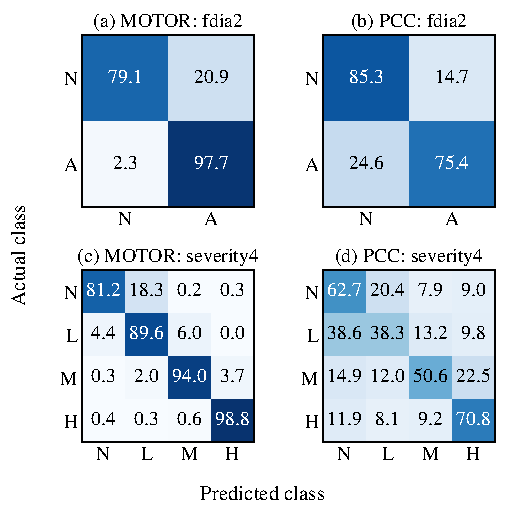
\includegraphics[width=\linewidth]{figs_revised/figure5_confusion_matrices.pdf}
\caption{Confusion matrices for validation-selected full-feature models. Rows denote actual classes and columns predicted classes. Percentages are row-normalized from pooled predictions across the three recording holdouts; repeated appearances of a recording are not independent physical replications. Table~\ref{tab:all_tasks_in_domain} instead averages per-repeat metrics.}
\label{fig:main_confusion_matrices}
\end{figure*}
\agent{Check my previous version of figure do exactly like that. find the source code generated that and use exactly the same thing. its visualization is much better. }
\begin{figure*}[t]
\centering
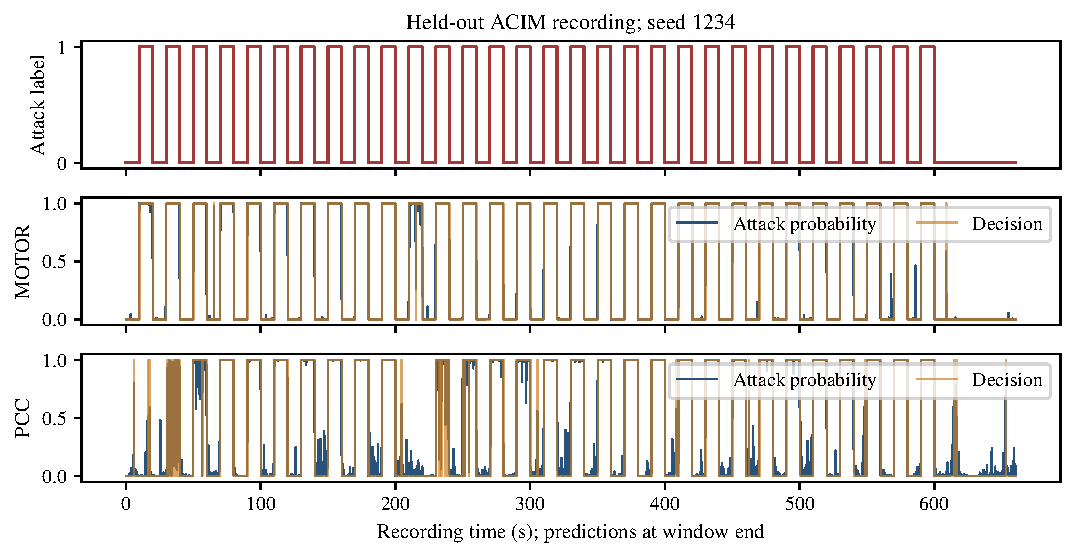
\includegraphics[width=\linewidth]{figs_revised/figure6_heldout_acim.pdf}
\caption{Binary detector outputs on the first alphabetic held-out ACIM recording for seed 1234, selected without inspecting performance. Predictions are placed at the end of each 0.2-s acquisition window. The full recording includes the zero-bias post-schedule interval; fluctuations and false alarms are shown without filtering.}
\label{fig:case1_30_motor_pcc_detection_examples}
\end{figure*}
\section{LATENCY AND REDUCED-FEATURE INFERENCE ANALYSIS}
\label{sec:realtime}
Practical PCC monitoring requires low latency and stable online throughput. This section reports per-window latency, throughput, pruning, and reduced-feature effects. In particular, the analysis focuses on end-to-end processing latency, online throughput, feature-pruning effects, and practical considerations for deployment at the PCC. 

\subsection{Inference Latency and Throughput on CPU/GPU}
\label{sec:latency_throughput}

Runtime was measured on the Intel Core Ultra 9 285K CPU and NVIDIA RTX 5090 GPU using the seed-1234 binary models. Each variant used 10 warm-up executions and 50 timed repetitions. The benchmark separates feature extraction, normalization/transfer/inference, and full processing, reporting median and 95th-percentile latency (Table~\ref{tab:runtime_latency}). End-to-end processing excludes the 200-ms acquisition window; it is not an attack-onset-to-alarm delay. CPU and GPU-assisted versions use the same selected models.

Full-feature GPU-assisted processing takes 22.37~ms for PCC and 66.33~ms for motor sensing, with 95th percentiles of 23.93 and 67.55~ms. Both measured processing times are below the 200-ms window interval. Reciprocal median processing rates are approximately 44.69 and 15.08 windows/s, respectively; these are workstation processing capacities, not measured embedded worst-case guarantees. Acquisition, scheduling, and any alarm-persistence logic must be included in a deployed timing budget.
\agent{bring this table in exactly previous version. just update numbers you can have median and 95th percentile column . your table structures are really hard for reviewers to follow. }
\begin{table*}[t]
\centering
\footnotesize
\caption{Full-feature processing latency, excluding 200-ms acquisition.}
\label{tab:runtime_latency}
\renewcommand{\arraystretch}{1.12}
\setlength{\tabcolsep}{3pt}
\begin{tabular}{lcccc}
\hline
Stream & Execution & Stage & Median (ms) & 95th pct. (ms) \\
\hline
PCC & CPU & Extraction & 21.59 & 21.88 \\
PCC & CPU & Norm./transfer/inference & 0.73 & 0.82 \\
PCC & CPU & Total processing & 22.32 & 22.66 \\
PCC & GPU-assisted & Extraction & 21.64 & 23.11 \\
PCC & GPU-assisted & Norm./transfer/inference & 0.72 & 0.85 \\
PCC & GPU-assisted & Total processing & 22.37 & 23.93 \\
MOTOR & CPU & Extraction & 65.68 & 66.64 \\
MOTOR & CPU & Norm./transfer/inference & 1.23 & 1.34 \\
MOTOR & CPU & Total processing & 66.87 & 67.88 \\
MOTOR & GPU-assisted & Extraction & 64.99 & 66.19 \\
MOTOR & GPU-assisted & Norm./transfer/inference & 1.33 & 1.42 \\
MOTOR & GPU-assisted & Total processing & 66.33 & 67.55 \\
\hline
\end{tabular}

\end{table*}

\subsection{Feature Pruning for Low-Latency Anomaly Detection}
\label{sec:feature_pruning}

Binary-model features were ranked by validation-set permutation importance: the decrease in balanced accuracy when one feature trajectory is permuted across validation windows, repeated three times. Test labels were not used for ranking. Within each split, global top-75\%, top-50\%, and top-25\% subsets and per-channel top-15/top-10 subsets were retrained with the full model's selected architecture and training protocol. Fig.~\ref{fig:top10_feature_importance} summarizes validation importance across repeats; correlated features can share predictive information, so these scores do not identify causal attack mechanisms.

Table~\ref{tab:feature_pruning_anomaly2_runtime} shows that fewer retained features do not guarantee faster extraction. The PCC top-25\% subset retains 18 of 74 features and approximately preserves balanced accuracy (80.29\%), but processing remains 22.42~ms versus 22.37~ms for full features. The motor top-25\% subset retains 56 of 222 features, gives 86.83\% balanced accuracy versus 88.26\% for full input, and reduces processing from 66.33 to 56.41~ms (1.18$\times$). Selective extraction must still compute shared spectral intermediates when retained features depend on them, which limits savings. All subsets are reported; no test-best subset replaces the primary full-feature model.
\agent{this figure is not good at all. check previous version figure. it had better colors and visualization. do the same thing but you can use the new line. I dont know what is the bar and line here. }
\begin{figure*}[t]
\centering
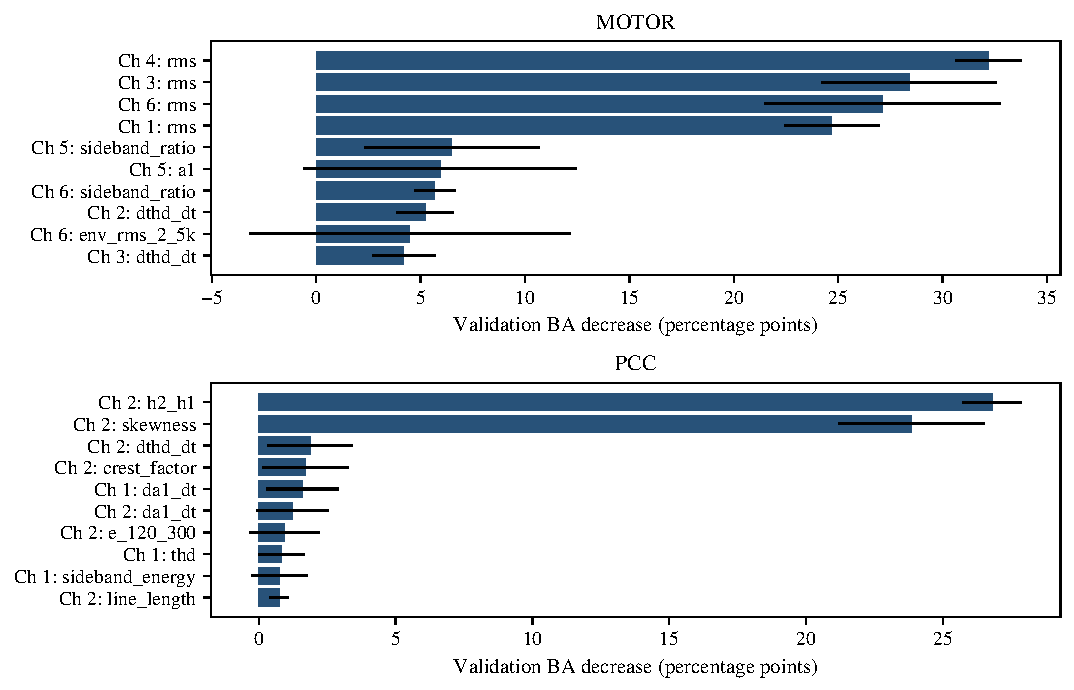
\includegraphics[width=\linewidth]{figs_revised/figure7_validation_feature_importance.pdf}
\caption{Top ten features by mean validation permutation-importance decrease in balanced accuracy. Error bars show SD across three recording splits. Channels 1--3 and 4--6 are ACIM and PMSM phase currents, respectively; PCC channels 1 and 2 are voltage and current. Importance supports feature ranking rather than a causal interpretation.}
\label{fig:top10_feature_importance}
\end{figure*}

\agent{the first comment is that use the same style of the my previous table. it was much better. specifically for PCC and motor column. make it row. Also I think the way you designed this test is wrong. what is the problem here is that with 25 percent of features extraction, I dont see any speedups. If we calculate less features it should be faster. find the source of problem. }
\begin{table*}[t]
\centering
\footnotesize
\caption{Binary feature pruning: mean $\pm$ SD performance and seed-1234 GPU-assisted processing.}
\label{tab:feature_pruning_anomaly2_runtime}
\renewcommand{\arraystretch}{1.12}
\setlength{\tabcolsep}{3pt}
\begin{tabular}{lccccccc}
\hline
Stream & Subset & Features & Bal. acc. (\%) & Macro F1 (\%) & Median (ms) & 95th pct. (ms) & Speedup \\
\hline
PCC & Full & 74 & $80.29\pm3.03$ & $80.42\pm2.96$ & 22.37 & 23.93 & 1.00 \\
PCC & Top 75\% & 56 & $78.28\pm3.07$ & $78.41\pm3.37$ & 22.46 & 24.83 & 1.00 \\
PCC & Top 50\% & 37 & $78.87\pm2.79$ & $79.10\pm2.97$ & 22.58 & 24.02 & 0.99 \\
PCC & Top 25\% & 18 & $80.29\pm2.14$ & $80.58\pm2.29$ & 22.42 & 23.43 & 1.00 \\
PCC & 15/channel & 30 & $77.59\pm4.75$ & $77.74\pm4.94$ & 22.49 & 22.94 & 0.99 \\
PCC & 10/channel & 20 & $80.47\pm2.79$ & $80.69\pm2.80$ & 22.68 & 29.62 & 0.99 \\
MOTOR & Full & 222 & $88.26\pm9.99$ & $87.23\pm11.39$ & 66.33 & 67.55 & 1.00 \\
MOTOR & Top 75\% & 166 & $87.95\pm11.38$ & $87.19\pm12.42$ & 67.02 & 68.80 & 0.99 \\
MOTOR & Top 50\% & 111 & $89.28\pm11.33$ & $88.20\pm12.87$ & 66.49 & 70.36 & 1.00 \\
MOTOR & Top 25\% & 56 & $86.83\pm10.93$ & $85.44\pm12.39$ & 56.41 & 57.21 & 1.18 \\
MOTOR & 15/channel & 90 & $92.10\pm9.71$ & $91.44\pm10.88$ & 62.13 & 65.19 & 1.07 \\
MOTOR & 10/channel & 60 & $88.18\pm9.28$ & $87.20\pm10.62$ & 56.77 & 58.14 & 1.17 \\
\hline
\end{tabular}

\end{table*}

\subsection{LF/HF/TD Ablation for Binary Anomaly Detection}
\label{sec:lfhf_ablation}

All seven LF/HF/TD combinations were evaluated by retraining with the selected full-feature architecture fixed within each task, stream, and split. Table~\ref{tab:lfhf_ablation_anomaly2} reports binary results. For PCC, LF+Time reaches 80.03\% balanced accuracy, close to the full input at 80.29\%, while reducing GPU-assisted processing from 22.37 to 12.32~ms (1.82$\times$). Thus, the measured marginal PCC benefit of HF features does not establish that their extra computation is necessary for binary detection on this dataset.

For motor sensing, time-only reaches 92.89\% balanced accuracy and HF+Time reaches 94.11\%, compared with 88.26\% for the full input. Time-only processing takes 16.28~ms (4.07$\times$ faster than full). HF-only performs poorly for both streams (63.76\% motor and 64.49\% PCC balanced accuracy), but its combination with time features is useful for motor sensing. These are observed ablation results, not test-based selection of a new primary model. Severity ablations and complete per-repeat measurements are supplied with the revision materials.
\agent{make the style like before. I liked that more. stream column. }
\begin{table*}[t]
\centering
\footnotesize
\caption{Binary LF/HF/TD ablation (mean $\pm$ SD, \%).}
\label{tab:lfhf_ablation_anomaly2}
\renewcommand{\arraystretch}{1.12}
\setlength{\tabcolsep}{3pt}
\begin{tabular}{lccccc}
\hline
Stream & Features & Number & Accuracy & Balanced acc. & Macro F1 \\
\hline
PCC & Full & 74 & $80.78\pm2.95$ & $80.29\pm3.03$ & $80.42\pm2.96$ \\
PCC & LF only & 36 & $74.03\pm3.84$ & $73.56\pm3.13$ & $73.59\pm3.33$ \\
PCC & HF only & 22 & $64.50\pm4.62$ & $64.49\pm4.56$ & $64.21\pm4.71$ \\
PCC & Time only & 16 & $72.18\pm1.73$ & $70.66\pm1.77$ & $70.65\pm1.76$ \\
PCC & LF + HF & 58 & $68.66\pm4.60$ & $68.15\pm4.26$ & $68.18\pm4.39$ \\
PCC & LF + Time & 52 & $80.49\pm1.73$ & $80.03\pm1.79$ & $80.16\pm1.73$ \\
PCC & HF + Time & 38 & $69.49\pm3.66$ & $67.85\pm3.11$ & $67.72\pm3.06$ \\
MOTOR & Full & 222 & $87.41\pm11.13$ & $88.26\pm9.99$ & $87.23\pm11.39$ \\
MOTOR & LF only & 108 & $81.61\pm3.08$ & $80.54\pm2.55$ & $80.94\pm2.77$ \\
MOTOR & HF only & 66 & $63.32\pm4.96$ & $63.76\pm4.28$ & $63.14\pm4.81$ \\
MOTOR & Time only & 48 & $92.61\pm5.51$ & $92.89\pm4.96$ & $92.58\pm5.50$ \\
MOTOR & LF + HF & 174 & $80.33\pm7.88$ & $79.91\pm7.06$ & $80.05\pm7.60$ \\
MOTOR & LF + Time & 156 & $90.70\pm8.32$ & $91.17\pm7.45$ & $90.65\pm8.35$ \\
MOTOR & HF + Time & 114 & $93.87\pm4.56$ & $94.11\pm4.04$ & $93.85\pm4.54$ \\
\hline
\end{tabular}

\end{table*}

\section{Discussion}
\label{sec:discussion}
\subsection{Why Adaptation Helps More in One Direction}
\label{sec:adaptation_asymmetry}

The PCC results retain a strong direction asymmetry: at 20\% target labels, PMSM-to-ACIM fine-tuning reaches 91.38\% balanced accuracy, while ACIM-to-PMSM reaches 56.30\%. Source-only predictions also show different class biases: for PCC ACIM-to-PMSM, the mean attack miss rate is 92.71\%; in the reverse direction the normal false-alarm rate is 86.03\%. These biases show that source-domain decision boundaries and operating distributions do not transfer reliably. They do not isolate a causal mechanism for the asymmetry.

The target-only comparison is essential. PCC PMSM-to-ACIM fine-tuning exceeds its matched target-only control, whereas motor ACIM-to-PMSM fine-tuning is worse than its control at 20\%. Source pretraining can therefore help or hinder adaptation under the stated budget. The results motivate target-domain calibration and direction-specific evaluation; they do not show that any pretrained motor model is suitable for another installation.

\subsection{PCC vs Motor Tradeoffs}
\label{sec:pcc_vs_motor}

Motor sensing provides higher mean class-balanced performance on this dataset, particularly for distinguishing injected-bias bins. PCC sensing reduces terminal instrumentation but aggregates the responses of both drive branches and their shared converter interface. For the four-class PCC model, relatively high any-attack recall at medium/high bias coexists with low exact-severity recall and frequent false alarms. The separate binary detector is the stronger primary PCC alarm model in these experiments.

The motor-type task is an auxiliary diagnostic of distinguishable recording domains, not proof of a causal motor-physics explanation: the motor families also have different load-setting ranges and share only one installation per family. Attack-only regression likewise estimates injected bias rather than torque or damage (Appendix~\ref{app:auxiliary_diagnostics}). For efficiency, the PCC LF+Time representation offers a measured alternative to full features with similar balanced accuracy. Neither classification scores nor processing latency alone establish safe automatic mitigation.

\subsection{Limitations}
\label{sec:limitations}

The evidence is limited to additive, piecewise-constant current-feedback bias on one two-branch laboratory platform. Monitoring sensors are assumed uncompromised; coordinated attacks on those sensors, replay, denial of service, command attacks, and stealthy time-varying perturbations were not tested. Three fixed speed settings and three load settings were recorded for each machine, but dedicated speed ramps, load steps, and other dynamic operating conditions were not evaluated. Brake excitation identifies operating settings; calibrated shaft torque and mechanical harm were not measured.

PCC signatures can depend on the shared rectifier, downstream inverter topology, control behavior, modulation, sensor transfer functions, and supply impedance. These factors were not varied independently in the dataset. Consequently, no robustness claim is made for other converter topologies, modulation strategies, grids, or installations. Whole-recording holdouts remove within-repeat recording/episode overlap, but remain a retrospective evaluation on reused data from the same apparatus. Three repeated holdouts do not provide independent hardware replication or a strong significance test.

The adaptation study requires target labels and uses fixed training budgets; unsupervised adaptation and exhaustive target-only optimization are outside its scope. PCC severity remains weak, and normal false alarms are material even when attack recall is high. Finally, measured workstation processing times exclude acquisition and do not establish embedded worst-case latency or a tested closed-loop mitigation system.
\agent{for this figure use the same format I have used in previous version. }
\begin{figure*}[t]
\centering
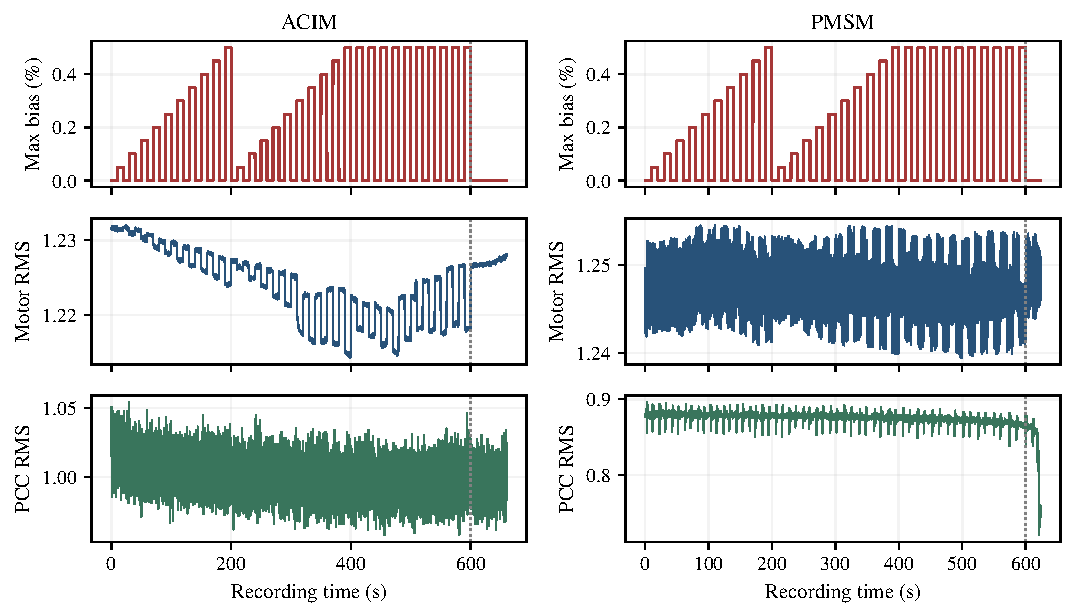
\includegraphics[width=\linewidth]{figs_revised/figure8_raw_rms.pdf}
\caption{Representative held-out ACIM and PMSM recordings. Top: documented maximum injected phase bias; middle/bottom: RMS of one motor-current and PCC-current channel in recorded acquisition units. The displayed interval covers the scheduled episodes and zero-bias tail. These traces illustrate operating responses, not calibrated torque, and their visual differences are not evidence of a causal transfer mechanism.}
\label{fig:app_attack_process_examples}
\end{figure*}

\section{Conclusion}
\label{sec:conclusion}

This paper assessed nonintrusive FDIA monitoring in a heterogeneous ACIM/PMSM inverter-fed drive platform using recording- and episode-disjoint evaluation. Across three holdouts, binary accuracy was 87.41\% for motor-side sensing and 80.78\% for PCC sensing. Four-class injected-bias balanced accuracy was 90.81\% and 55.62\%, respectively, demonstrating a substantial limitation of PCC severity estimation. Severity-conditioned attack recall complements exact-bin recall but must be interpreted alongside false alarms. Cross-motor source-only transfer was unreliable, and supervised adaptation benefits depended on direction and sensing location; matched target-only controls prevented attributing every gain to pretraining. PCC LF+Time retained approximately full-feature binary balanced accuracy while reducing processing from 22.37 to 12.32~ms on the tested workstation. The results support further development of PCC monitoring for additive feedback-bias attacks while delimiting its accuracy, calibration, and deployment constraints.

\bibliographystyle{ieeetr}
\bibliography{ref_revised}

\appendices
\section{Additional Experimental and Diagnostic Results}
\label{app:additional_results}


This appendix provides representative FDIA recordings, the extracted feature definitions, severity-conditioned detection metrics, hyperparameter sensitivity, and auxiliary bias regression. Complete numeric results and per-repeat configurations accompany the manuscript.

\subsection{Representative FDIA Episodes}
\label{app:fdia_episode_examples}

Figure~\ref{fig:app_attack_process_examples} shows representative consecutive FDIA episodes applied to the ACIM and PMSM drive systems. In both examples, the top panel shows the scheduled FDIA severity level, while the middle and bottom panels show the corresponding motor-current and PCC-current RMS responses over each complete recording, including the normal post-schedule tail. RMS is computed over each 2,000-sample outer window for these descriptive plots. It must be distinguished from the TD RMS feature, which uses 500-sample subwindows, and from HF band-limited RMS.


\subsection{Extracted Feature Set}
\label{app:feature_set}

Table~\ref{tab:app_extracted_features} summarizes the extracted features used in the proposed LF/HF/TD pipeline. Each channel is represented using low-frequency spectral features, high-frequency spectral-envelope features, and time-domain statistical features.

\begin{table}[t]
\centering
\scriptsize
\caption{Extracted features per channel in the proposed LF/HF/TD pipeline.}
\label{tab:app_extracted_features}
\setlength{\tabcolsep}{3pt}
\renewcommand{\arraystretch}{1.08}
\begin{tabularx}{\columnwidth}{l c c X}
\hline
Type & No. & Window / Stride & Features \\
\hline
LF & 18 & 500 / 25 &
$A_1$, $f_1$, $\phi_1$, THD, $H_2/H_1$, $H_3/H_1$, $H_5/H_1$, $H_7/H_1$,
$\phi_3-\phi_1$, $\phi_5-\phi_1$, sideband energy/ratio,
$E_{0-120}$, $E_{120-300}$, $E_{300-500}$,
$df_1/dt$, $dA_1/dt$, $d\mathrm{THD}/dt$ \\
\hline
HF & 11 & 250 / 29 &
RMS$_{2-5k}$, energy ratio, centroid, bandwidth, flatness, kurtosis,
peak frequency, peak-to-band, envelope RMS, envelope kurtosis, envelope crest factor \\
\hline
TD & 8 & 500 / 25 &
RMS, standard deviation, crest factor, kurtosis, skewness, peak-to-peak, line length, Teager MAV \\
\hline
Total & 37 & -- & LF (18), HF (11), TD (8) \\
\hline
\end{tabularx}
\end{table}


\subsection{Severity-Conditioned Attack Detection}
\label{app:severity_detection}
Table~\ref{tab:severity_detection_recall} separates correct bias-bin classification from detecting any attack. The repeated false-alarm entries belong to the same four-class model and do not depend on the actual attack level. Fig.~\ref{fig:severity_detection_decisions} presents the corresponding PCC decision matrices; pooled normal recall can differ slightly from the mean per-repeat recall because normal-window counts vary across holdouts.

\begin{table*}[t]
\centering
\footnotesize
\caption{Four-class models: exact-severity recall, any-attack recall, and normal false alarms (mean $\pm$ SD, \%).}
\label{tab:severity_detection_recall}
\renewcommand{\arraystretch}{1.12}
\setlength{\tabcolsep}{3pt}
\begin{tabular}{lcccc}
\hline
Stream & True bias & Exact recall & Any-attack recall & Normal false alarms \\
\hline
MOTOR & Low & $89.58\pm2.14$ & $95.58\pm4.15$ & $19.08\pm16.08$ \\
MOTOR & Medium & $93.96\pm1.05$ & $99.71\pm0.04$ & $19.08\pm16.08$ \\
MOTOR & High & $98.76\pm0.27$ & $99.65\pm0.29$ & $19.08\pm16.08$ \\
PCC & Low & $38.33\pm7.04$ & $61.39\pm2.64$ & $37.23\pm3.17$ \\
PCC & Medium & $50.58\pm7.01$ & $85.08\pm6.52$ & $37.23\pm3.17$ \\
PCC & High & $70.79\pm2.28$ & $88.09\pm7.22$ & $37.23\pm3.17$ \\
\hline
\end{tabular}

\end{table*}
\begin{figure*}[t]
\centering
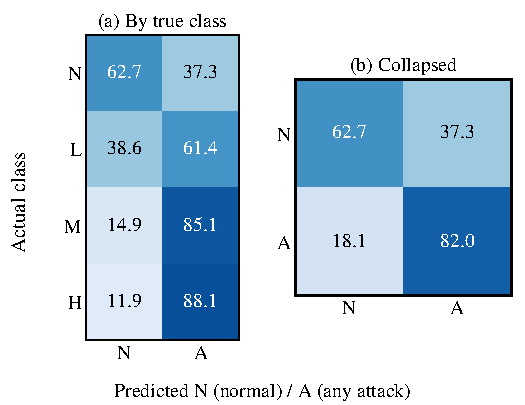
\includegraphics[width=\linewidth]{figs_revised/pcc_severity_and_detection_confusions.pdf}
\caption{PCC severity model evaluated as (a) exact four-class predictions, (b) normal/any-attack decisions for each actual bias class, and (c) a collapsed binary confusion matrix. Percentages pool the three holdouts and normalize each row. Panel (c) is derived from the severity model, not the separately trained binary detector.}
\label{fig:severity_detection_decisions}
\end{figure*}
\subsection{Hyperparameter Sensitivity}
\label{app:sensitivity}
Fig.~\ref{fig:hyperparameter_sensitivity} reports all one-factor perturbations. PCC binary mean balanced accuracy ranges from 72.23\% to 78.33\% among these variants, compared with 80.29\% for the selected reference. PCC severity varies from 51.25\% to 55.71\%, compared with 55.62\%. Motor severity is more sensitive to the high learning rate, falling to 77.69\% mean balanced accuracy. Therefore, the comparison supports a persistent PCC severity limitation rather than insensitivity to every training setting.

\begin{figure*}[t]
\centering
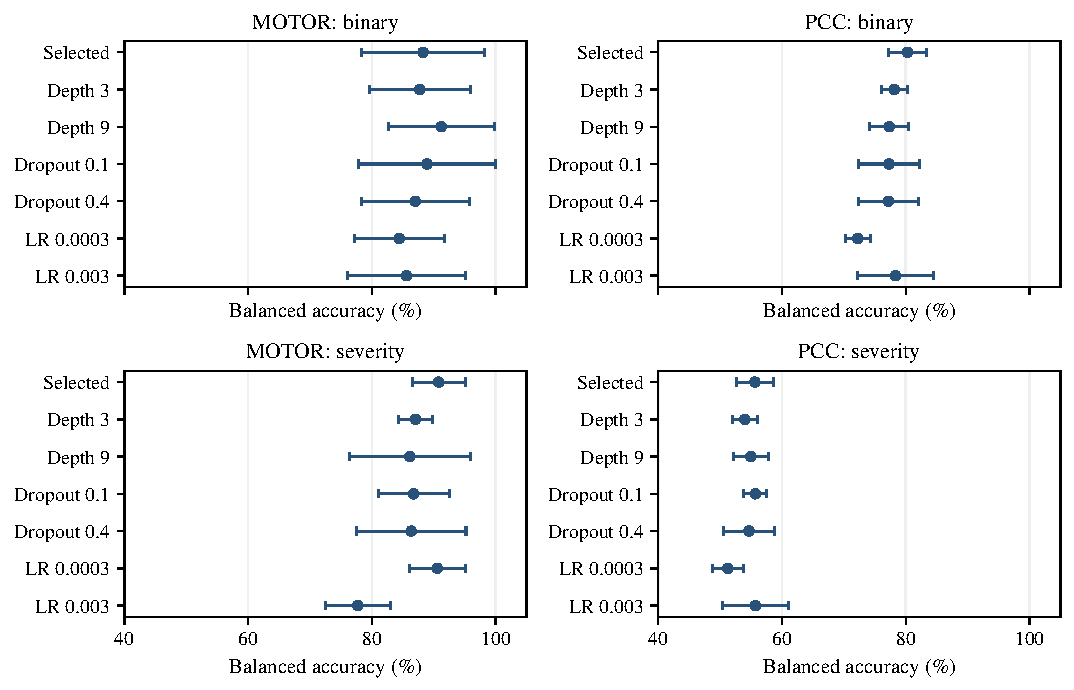
\includegraphics[width=\linewidth]{figs_revised/hyperparameter_sensitivity.pdf}
\caption{One-factor sensitivity around the validation-selected full-feature configuration in each repeat. Error bars indicate sample SD across three recording holdouts. Only the named hyperparameter changes; the selected reference can differ across tasks, streams, and repeats.}
\label{fig:hyperparameter_sensitivity}
\end{figure*}
\subsection{Auxiliary Diagnostic Tasks}
\label{app:auxiliary_diagnostics}
\agent{do we have any figure from the regression results? I think it is good to add here. }
The motor-type results are included in Table~\ref{tab:all_tasks_in_domain}. For attack-only regression, the target is $100\|\boldsymbol{\alpha}\|_\infty$, in percentage points of nominal current-feedback bias. A scalar output replaces the classification head; training uses Smooth-L1 loss with transition parameter 0.5 and validation mean absolute error (MAE) for checkpoint selection. The severity-selected architecture is retained within each stream and repeat. Motor-side MAE is $0.0196\pm0.0041$ percentage points, with mean $R^2=0.961$; PCC MAE is $0.0981\pm0.0049$ percentage points, with mean $R^2=0.267$. These are estimates of injected amplitude on attacked windows, not measured mechanical impact.

\end{document}

